\chapter{تشغيل الصوت بـ\textenglish{FMOD}}

منذ أن اكتشفنا الـ\textenglish{SDL}،
تعلّمنا موضعة صور على النافذة، التفاعل مع المُستعمل بالفأرة و لوحة المفاتيح، كتابة نصوص، لكن ينقص أمر بالتأكيد : الصوت !

سيسدّ هذا الفصل ذلك النقص. بما أن الإمكانيّات التي توفّرها لنا الـ\textenglish{SDL}
من ناحية الصوت محدودة جداً، سنكتشف هنا مكتبة متخصصة في الصوت :
\textenglish{FMOD}.

\section{تثبيت \textenglish{FMOD}}

\subsection{لماذا \textenglish{FMOD} ؟}

أنت تعرف ذلك الآن : الـ\textenglish{SDL}
ليست فقط مكتبة رسومية. هي تسمح أيضاً بمعالجة الصوت عن طريق وحدة تسمّى
\textenglish{SDL\_audio}.
فلماذا إذاً سنحضّر مكتبة خارجية لا علاقة لها بالـ\textenglish{SDL}
كـ\textenglish{FMOD} ؟

في الواقع هو اختيار قمتُ به بعد عدّة اختبارات. كان بإمكاني أن أشرح لك طريقة معالجة الصوت بالـ\textenglish{SDL}
لكنّي فضّلت عدم فعل ذلك.\\
سأشرح موقفي أكثر.

\subsection{لماذا قمتُ بتجنّب \textenglish{SDL\_audio} ؟}

يعتبر التحكم في الصوت بالـ\textenglish{SDL}
"منخفض المستوى". هذا يعني أنه يجب القيام بالعديد من التعامُلات الدقيقة كي نستطيع تشغيل الصوت. بمعنى آخر، سيكون الأمر صعباً و لا أجد ذلك ممتعاً. توجد مكتبات أخرى تسمح بتشغيل الصوت بشكل بسيط.

\begin{information}
تذكير بسيط : مكتبة "منخفضة المستوى" هي مكتبة قريبة من الحاسوب. يجب أن نتعرّف إذا على قليل من العمل الداخلي للحاسوب كي نستفيد منها و يتطلب الأمر في الواقع وقتاً أكثر من الوقت اللازم للقيام بنفس الشيء مع مكتبة "عالية المستوى".\\
لا تنس أنّ كلّ شيء نسبيّ : لا توجد مكتبات منخفضة المستوى من جهة و أخرى عالية المستوى من جهة أخرى. هي فقط أكثر أو أقل من بعضها البعض في المستوى. مثلا، المكتبة
\textenglish{FMOD}
عالية المستوى مقارنة بالوحدة
\textenglish{SDL\_audio}
من الـ\textenglish{SDL}.
\end{information}

تفصيل آخر مهم، تسمح الـ\textenglish{SDL}
بتشغيل صوت بصيغة
\textenglish{WAV}
فقط. صيغة الصوت هذه ليست مضغوطة. أي أن موسيقى من 3 دقائق تأخذ عشرات الميغا أوكتي،
على عكس الصيغ المضغوطة مثل
\textenglish{MP3}
أو
\textenglish{Ogg}
التي تحجز حجم ذاكرة أقلّ بكثير (من 2 إلى 3 ميغا أوكتي).

في الواقع، لو نفكّر في الأمر جيًداً، كان الأمر مشابهاً بالنسبة للصور، فالـ\textenglish{SDL}
لا تتعامل إلا مع الصيغة
\textenglish{BMP}
(صُور غير مضغوطة) بشكل مبدئي. مما استوجب علينا تسطيب مكتبة إضافية و هي
\textenglish{SDL\_image}
لنتمكّن من قراءة صيغ الصور الأخرى كـ\textenglish{JPEG}، \textenglish{PNG}، \textenglish{GIF}،
إلخ.

اعلم أنه هناك مكتبة مكافئة بالنسبة للصوت و هي :
\textenglish{SDL\_mixer}.
هي قادرة على قراءة عدد كبير من صيغ الصوت، من بينها
\textenglish{MP3}، \textenglish{Ogg}، \textenglish{Midi} \dots
و رغم ذلك، لم أكلّمك عن هذه المكتبة. لماذا ؟

\subsection{لماذا قمتُ بتجنّب \textenglish{SDL\_mixer} ؟}

\textenglish{SDL\_mixer}
هي مكتبة نضيفها للـ\textenglish{SDL}،
بطريقة 
\textenglish{SDL\_image}.
هي سهلة للاستعمال و تقرأ العديد من صيغ الصوت المختلفة. لكن، و بعد الاختبارات التي قمتُ بها، تبيّن لي أن هذه المكتبة تحتوي عِلَلا مزعجة بالإضافة إلى كونها محدودة من ناحية المزايا التي تمنحها.

من أجل هذه الأسباب توجّهت مباشرة إلى
\textenglish{FMOD}،
مكتبة لا علاقة لها بالـ\textenglish{SDL}
بالتأكيد، لكن لها الأفضلية كونها قوية و متداولا عليها.

\subsection{تنزيل \textenglish{FMOD}}

إن كنت قد حكيت لك كل هذا، فهذا فقط لأخبرك بأن اختيار
\textenglish{FMOD}
لم يكن عشوائياً. ببساطة هي أفضل مكتبة مجانية استطعت إيجادها.\\
كما أنها سهلة الاستخدام كـ\textenglish{SDL\_mixer}
بأفضلية لا يمكن تجاهلها : لا توجد بها عِلَل برمجية.

تسمح
\textenglish{FMOD}
بالقيام بالعديد من الوظائف التي لا تسمح بها
\textenglish{SDL\_mixer}،
كالتأثيرات الصوتيّة ثلاثية الأبعاد.

\begin{warning}
\textenglish{FMOD}
هي مكتبة مجانية لكن ليست تحت رخصة
\textenglish{LGPL}
على عكس الـ\textenglish{SDL}.
هذا يعني أنه بإمكانك أن تستخدمها مادامت لم تحقق بها برامج مدفوعة. إذا أردت أن يكون البرنامج غير مجاني، يجب أن تدفع رسوماً لمؤلّف المكتبة (سأتركك تطّلع على الأسعار من خلال الموقع الرسمي لـ\textenglish{FMOD}).\\
كثير من الألعاب التجارية تستعمل
\textenglish{FMOD}
و من أشهر هذه الألعاب :
\textenglish{Starcraft II}، \textenglish{World of Warcraft : Cataclysm}، \textenglish{Crysis 2}،
إلخ.
\end{warning}

تتوفر العديد من نسخ
\textenglish{FMOD}،
و النسخة الموجهّة إلى الاستعمال في أنظمة التشغيل المألوفة
(\mbox{\textenglish{GNU/Linux}}، \textenglish{Windows}، \mbox{\textenglish{Mac OS X}}، \dots)
تُدعى
\textenglish{FMOD Ex Programmers API}.

نزّل إذا نسخة
\textenglish{FMOD Ex}
المناسبة لنظام التشغيل الخاص بك. خذ النسخة المسمّاة "مستقرة"
(\textenglish{stable}).

و تأكد بشكل خاص ما إن كان لديك نظام تشغيل
\textenglish{32 bits}
أو
\textenglish{64 bits}
(في
\textenglish{Windows}،
 قم بنقر يميني على جهاز الكمبيوتر
(\textenglish{Computer})
ثم في قسم الخصائص
(\textenglish{Properties})
تجد المعلومة اللازمة).

\url{http://www.fmod.org/fmod-downloads.html#FMODExProgrammersAPI}

\subsection{تثبيت \textenglish{FMOD}}

يعمل التثبيت بنفس مبدأ عمل المكتبات السابقة، أي مثل الـ\textenglish{SDL}.

يجدر بالملف الذي حمّلته أن يكون ملفاً تنفيذياً (في
\textenglish{Windows})،
 أو أن يكون أرشيفا 
(\InlineCode{.dmg}
في
\mbox{\textenglish{Mac OS X}}
و
\InlineCode{.tar.gz}
في
\mbox{\textenglish{GNU/Linux}}).

\begin{enumerate}
	\item ثبّت
	\mbox{\textenglish{FMOD Ex}}
على قرصك الصلب. الملفات التي نحتاجها يجب أن تتواجد في مجلّد يشبه هذا :\\
	\InlineCode{C:\textbackslash Program Files\textbackslash FMOD SoundSystem\textbackslash FMOD Programmers API Win32\textbackslash api}.
	\item في هذا المجلّد تجد الـ\textenglish{DLL}
	الخاصّ بـ\mbox{\textenglish{FMOD Ex}}
	(\InlineCode{fmodex.dll})
	و يجب أن يوضع في مجلّد المشروع. الـ\textenglish{DLL}
	الأخرى، أي
	\InlineCode{fmodexL.dll}
	تعمل على تنقيح العلل البرمجية. لن نقوم بذلك هنا. تذكّر فقط بأن الملف
	\InlineCode{fmodex.dll}
	هو الذي يجب أن تُعطيه مع الملف التنفيذي للبرنامج.
	\item في المجلّد
	\InlineCode{api/inc}،
	تجد الملفات
	\InlineCode{.h}.
	ضعها كلّها إلى جانب الملفات الرأسية التي هي في مجلّد البيئة التطويرية. مثلا :
	\InlineCode{Code Blocks/mingw32/include/fmodex}
	(لقد أنشأت مجلّدا خصيصاً لأجل
	\textenglish{FMOD}
	كما مثل الـ\textenglish{SDL}).
	\item في المجلّد
	\InlineCode{api/lib}،
	استرجع الملف الموافق للمترجم. يجدر بملف نصّي أن يشير إلى أي ملف يجب أن نأخذ.
	\begin{itemize}
		\item إذا كنت تستعمل
		\textenglish{Code::Blocks}،
		فالمترجم هو
		\textenglish{mingw}.
		أنسخ الملف
		\InlineCode{libfmodex.a}
		في المجلّد
		\InlineCode{lib}
		للبيئة التطويرية.
		
		في
		\textenglish{Code::Blocks}،
		إنه المجلّد
		\InlineCode{CodeBlocks/mingw32/lib}.
		\item إذا كنت تستعمل
		\textenglish{Visual C++}،
		استرجع الملف
		\InlineCode{fmodex\_vc.lib}.
	\end{itemize}
	\item أخيراً، الشيء الأكثر أهمية ربّما، يوجد مجلّد 
	\InlineCode{documentation}
	في المجلّد
	\textenglish{FMOD Ex}.
	من المفروض أن تتم إضافة اختصارات إلى قائمة "إبدأ" نحو هذه الملفات التوجيهية. أبق نظرك عليها لأنه لا يمكننا أن نكتشف كلّ ميزات
	\textenglish{FMOD Ex}
	في هذا الفصل. ستحتاج إلى هذه الملفات في أقرب الآجال بالتأكيد.
	
	يبقى أن نخصص المشروع. هنا أيضاً و مثل كلّ مرة : افتح المشروع بواسطة البيئة التطويرية المفضّلة و أضف الملف
	\InlineCode{.a}
	(أو
	\InlineCode{.lib})
	إلى قائمة الملفات التي يجب أن يسترجعها محرر الروابط.\\
	في
	\textenglish{Code::Blocks}
	(يخالجني شعور بأنني أقوم بالتكرار)، إذهب إلى قائمة
	\InlineCode{Project} / \InlineCode{Build Options}
	ثم قسم
	\InlineCode{Linker}،
	أنقر على
	\InlineCode{Add}
	و أشر إلى المسار الذي يوجد به الملف
	\InlineCode{.a}
	إذا ظهرت لك الرسالة~:
	"\textenglish{Keep as a relative path ?}"،
	أنصحك بأن تجيب بالسلب لكن يجدر بالأمور أن تشتغل في كلتا الحالتين.
	
	تم تثبيت
	\textenglish{FMOD Ex}،
	فلنَرَى بسرعة مما هي مُشَكَّلَة.
\end{enumerate}

\section{تهيئة و تحرير غرض نظامي}

المكتبة
\textenglish{FMOD Ex}
متوفّرة من أجل اللغتين
\textenglish{C}
و
\textenglish{C++}.\\
الشيء الخاص فيها هو أن مطوّري هذه المكتبة احتفظوا ببعض التناسق في "تركيب الكلمات"
(\textenglish{Syntax})
بين اللغتين. الميزة الأولى هي أنه إذا تعلّمت التعامل مع
\textenglish{FMOD Ex}
في لغة الـ\textenglish{C}
ستتمكن من فعل ذلك في الـ\textenglish{C++}
بنسبة 95\%.

\subsection{تضمين الملف الرأسي}

قبل كلّ شيء، يلزمك أن تقوم بتضمين الملف الرأسي الخاص بـ\textenglish{FMOD}.
 لابأس في التذكير بكتابته :

\begin{Csource}
#include <fmodex/fmod.h>
\end{Csource}

لقد وضعت هذا الملف في المجلّد الداخلي
\InlineCode{fmodex}.
عدّل على هذا السطر من الشفرة على حسب المسار الذي يتواجد به الملف عندك.\\
إذا كنت تعمل على
\mbox{\textenglish{GNU/Linux}}،
 يجدر بالتسطيب أن يتم تلقائيّا في المجلّد
\InlineCode{fmodex}.

\subsection{إنشاء و تهيئة غرض نظامي}

الغرض النظامي هو عبارة عن متغير نستفيد منه على طول البرنامج لكي نعرّف معاملات المكتبة.\\
تذكّر أنه بالـ\textenglish{SDL}
مثلاً، كان يجب أن نهيّئ المكتبة بشكل مباشر بواسطة دالة. هنا، دليل الاستعمال مختلف قليلاً : في عوض تهيئة كلّ المكتبة، لن نعمل إلا بغرض
(\textenglish{Object})
دوره تعريف سلوك هذه الأخيرة.

لكي ننشئ غرضا نظاميا، يكفي أن نعرّف مؤشّرا من نوع
\InlineCode{FMOD\_SYSTEM}.
مثلا :

\begin{Csource}
FMOD_SYSTEM *system;
\end{Csource}

لكي نحجز مكاناً في الذاكرة من أجل هذا الغرض النظامي، نستعمل الدالة
\InlineCode{FMOD\_System\_Create}
و التي نموذجها هو الآتي :

\begin{Csource}
FMOD_RESULT FMOD_System_Create(FMOD_SYSTEM ** system);
\end{Csource}

لاحظ أن هذه الدالة تأخذ مؤشّرا نحو مؤشّر يؤشّر نحو
\InlineCode{FMOD\_SYSTEM}.
القرّاء الأكثر حرصاً كانوا قد لاحظوا أنه لدى تعريف المؤشّر
\InlineCode{FMOD\_SYSTEM}،
لم يتم حجزه بواسطة
\InlineCode{malloc}
أو أي دالة أخرى. لهذا السبب تماماً تأخذ الدالة
\InlineCode{FMOD\_SYSTEM}
معاملا من ذلك النوع لكي تحجز مكاناً للمؤشّر النظامي.

بعد تعريف الغرض النظامي ، تكفي كتابة :

\begin{Csource}
FMOD_SYSTEM *system;
FMOD_System_Create(&system);
\end{Csource}

هكذا إذا، بما أننا نتوفّر الآن على الغرض النظامي، لم يتبّق علينا سوى تهيئته. لفعل هذا، نستعمل الدالة
\InlineCode{FMOD\_System\_Init}
ذات النموذج :
\begin{Csource}
FMOD_RESULT FMOD_System_Init(
	FMOD_SYSTEM *  system,
	int  maxchannels,
	FMOD_INITFLAGS  flags,
	void *  extradriverdata
);
\end{Csource}

\begin{itemize}
	\item المعامل
	\InlineCode{system}
	هو المعامل الذي يهمّنا أكثر، لأنه المؤشّر الذي سنقوم بتهيئته.
	\item المعامل
	\InlineCode{maxchannels}
	يمثّل العدد الأقصى للقنوات التي يجب أن تديرها
	\InlineCode{FMOD}.
	بمعنى آخر، هو العدد الأقصى للأصوات التي يمكن أن يتم تشغيلها في نفس الوقت. هذا يعتمد على قوة بطاقة الصوت لديك . ننصح عادة بقيمة 32 (قيمة كافية من أجل معظم الألعاب البسيطة). لمعلوماتك، يمكن نظرياً لـ\InlineCode{FMOD}
	إدارة 1024 قناة مختلفة، لكن بهذا المستوى ستخاطر بجعل حاسوبك يشتغل كثيرا !
	\item المعامل
	\InlineCode{flag}
	لا يهمّنا كثيراً في هذا الفصل، سنكتفي بإعطائه القيمة
	\InlineCode{FMOD\_INIT\_NORMAL}.
	\item المعامل
	\InlineCode{extradriverdata}
	لا يهمّنا أيضاً، سنعطيه القيمة
	\InlineCode{NULL}.
\end{itemize}

مثلا، لكي نعرّف، نحجز، و نهيّئ غرضا نظاميا،  نقوم بكتابة التالي :

\begin{Csource}
FMOD_SYSTEM *system;
FMOD_System_Create(&system);
FMOD_System_Init(system, 2, FMOD_INIT_NORMAL, NULL);
\end{Csource}

نتوفّر الآن على غرض نظامي جاهز للإستعمال.

\subsection{غلق و تحرير غرض نظامي}

نغلق ثمّ نحرر الغرض النظامي بواسطة دالتين :

\begin{Csource}
FMOD_System_Close(system);
FMOD_System_Release(system);
\end{Csource}

هل يجدر بي أن أعلّق على هذه الشفرة ؟

\section{الأصوات القصيرة}

فلنبدأ بدراسة الأصوات قصيرة المدّة.\\
"الصوت القصير"  كما أسمّيه، هو صوت يستمرّ غالباً بضعة ثوانٍ (أحياناً أقل من ثانية) و غالباً ما يُوجه للاستعمال المنتظم.

أمثلة عن أصوات قصيرة :

\begin{itemize}
	\item صوت إطلاق رصاصة.
	\item صوت مشي اللاعب.
	\item صوت 
	\textenglish{tic-tac}
	(لكيّ نوتّر اللاعب قبل انتهاء العد العكسي).
	\item صوت التصفيق.
	\item إلخ.
\end{itemize}

باختصار، كل صوت لا يعتبر موسيقى.\\
بشكل عام، هذه الأصوات قصيرة المدة إلى درجة أنه لا نحتاج إلى ضغطها. نجدها إذا في غالب الأحيان بصيغة
\textenglish{WAV}
غير مضغوطة.

\subsection{إيجاد الأصوات القصيرة}

 قبل أن نبدأ، سيكون من الجيد أن نتعرّف على بعض المواقع التي تقترح بنوكاً من الأصوات. بالفعل، لا أحد يريد أن يبدأ في تسجيل الأصوات بنفسه في المنزل.
 
سيكون الأمر جيداً فالأنترنت تقترح أصواتا قصيرة، غالباً بصيغة 
\textenglish{WAV}.\\
أين نجدها ؟ قد يبدو الأمر سخيفاً، لا يجب علينا أن نفكّر في ذلك (مع أنه لازم)، لكن
\textenglish{Google}
صديقنا. بشكل عشوائي، أكتب : 
"\textenglish{Free Sounds}"
و التي تعني "أصوات مجانية" بالإنجليزيّة، ستظهر لي ملايين النتائج.

لا شيء تحتاجه أكثر من الصفحة الأولى للبحث، ستجد ضالّتك هناك.\\
شخصياً حفظت الموقع 
\href{http://www.findsounds.com/}{\textenglish{FindSounds.com}}،
محرّك بحث متخصص في الأصوات. لا أدري إن كان الأفضل، لكن على أي حال هو موقع كامل.

\begin{information}
إذا لم تعرف  ماهي الكلمات المفتاحية التي تستعملها في البحث، توجّه إلى الصفحة الخاصة بأمثلة عن الكلمات المفتاحية للبحث.
يجب عليك أن تجيد بعض الكلمات الإنجليزية بالتأكيد (لكن على أي حال إن كنت تريد أن تصبح مبرمجاً، كيف ستفعل لو أنك لا تجيد على الأقل اللغة الإنجليزية ؟).
\end{information}

بالبحث عن كلمة
"\textenglish{gun}"،
سنجد أطنانا من أصوات إطلاق النار بالبندقية، لو نكتب
"\textenglish{door}"
سنجد أصوات تحرّك الباب (الصورة التالية)، إلخ.

\begin{figure}[H]
	\centering
	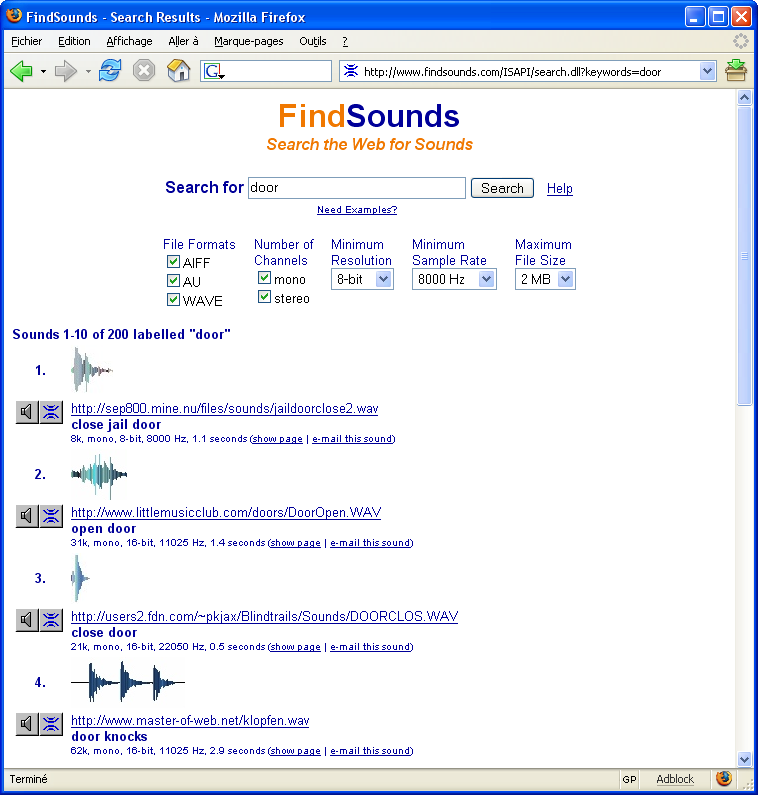
\includegraphics[height=0.4\textheight]{Chapter_III-8_FindSounds}
\end{figure}

\subsection{الخطوات التي يجب إتّباعها لتشغيل الصوت}

 الخطوة الأولى تنصّ على تحميل الصوت الذي نريد تشغيله في الذاكرة.\\
أنصحك بتحميل كلّ الأصوات التي ترى أنك ستستعملها كثيراً منذ بداية البرنامج. تقوم بتحريرها في النهاية. في الواقع، ما إن يتم تحميل الصوت في الذاكرة، ستكون قراءته سريعة جداً.

\subsubsection{المؤشّر}

الخطوة الأولى : إنشاء المؤشّر من نوع
\InlineCode{FMOD\_SOUND}
و الذي يمثّل الصوت.

\begin{Csource}
FMOD_SOUND *fire = NULL;
\end{Csource}

\subsubsection{تحميل الصوت}

الخطوة الثانية : تحميل الصوت بواسطة الدالة
\InlineCode{FMOD\_System\_CreateSound}.
هي تأخذ \dots خمسة معاملات :

\begin{itemize}
	\item \textbf{الغرض النظامي}
	 الذي تحدّثنا عنه سابقاً.
	
	بالطبع يجب أن يكون هذا الغرض جاهزاً للاستعمال (معرّفا، محجوزاً و مهيّئاً).
	\item \textbf{اسم الملف الصوتي}
	الذي نريد تحميله. يمكن أن يكون ذو صيغة
	\textenglish{WAV}، \textenglish{MP3}، \textenglish{OGG}،
	إلخ. من المستحسن دائماً أن يتم تحميل أصوات قصيرة (بضع ثوانٍ كحدّ أقصى) على أن يتم تحميل أصوات طويلة. في الواقع، تحمّل الدالة و تفك تشفير كلّ الصوت في الذاكرة، مما قد يأخذ مكانا كبيرا لو أن الصوت هو موسيقى !
	\item المعامل الثالث هو عَلم. 
	
	يهمّنا بشكل خاص هنا لأنه بفضله يمكننا أن نقول لـ\textenglish{FMOD}
	أن الصوت الذي ستشّغله هو عبارة عن صوت قصير. من أجل هذا نستعمل القيمة
	\InlineCode{FMOD\_CREATESAMPLE}.
	\item و الرابع لا يهمّنا، سنعطيه القيمة 
	\InlineCode{NULL}.
	\item المعامل الأخير هو من نوع
	\InlineCode{FMOD\_SOUND ** sound}،
	و هذا المؤّشر سنستعمله لاحقاً من أجل تشغيل الصوت.
	
	بشكل ما، يمكننا القول بأن هذا المؤشّر سيؤشّر على الصوت الذي نريد تشغيله.
\end{itemize}

 هذا مثال عن تحميل :

\begin{Csource}
FMOD_System_CreateSound(system, "pan.wav", FMOD_CREATESAMPLE, 0, &fire);
\end{Csource}

هنا، أقوم بتحميل الصوت
\InlineCode{pan.wav}.
المؤشّر
\InlineCode{fire}
سيعتبر كمرجع للصوت لاحقاً.

\begin{information}
 إذا كنت تريد أن تختبر الشفرات في نفس الوقت الذي أعطيها لك، أنصحك بتنزيل الصوت
\InlineCode{pan.wav}\\
 (\url{http://www.siteduzero.com/uploads/fr/ftp/mateo21/pan.wav})\\
 و الذي سأستعمله أيضاً في بقيّة هذا الفصل.
\end{information}

إذا اشتغل كلّ شيء على ما يُرام، تُرجع الدالة القيمة
\InlineCode{FMOD\_OK}
و إلا، فهذا يعني أنه حدث مشكل خلال فتح الملف الصوتي (ملف تالف أو غير موجود مثلا).

\subsubsection{تشغيل الصوت}

تريد تشغيل الصوت ؟ لا يوجد مشكل مع الدالة
\InlineCode{FMOD\_System\_PlaySound} !\\
يكفي أن تعطيها غرضا نظاميا جاهزا للاستعمال، رقم القناة التي نريد أن يُلعب فيها الصوت و أيضاً المؤشّر نحو الصوت، إضافة إلى معاملات أخرى لا تهمّنا سنعطيها القيمة
\InlineCode{NULL}
أو 0. بالنسبة لرقم القناة، لا تشغل بالك بالتفكير و ابعث القيمة
\InlineCode{FMOD\_CHANNEL\_FREE}
و اترك
\textenglish{FMOD}
تتحكّم في ذلك.

\begin{Csource}
FMOD_System_PlaySound(system, FMOD_CHANNEL_FREE, fire, 0, NULL);
\end{Csource}

\subsubsection{تحرير الصوت من الذاكرة}

حينما تصبح غير محتاجٍ للصوت، يجب عليك تحريره. \\
لا يوجد ما هو أسهل، يكفي أن تشير إلى المؤشّر الذي تريد تحريره بواسطة الدالة
\InlineCode{FMOD\_Sound\_Release}.


\subsection{مثال : لعبة إطلاق النار}

الأفضل الآن هو أن نلخّص كل ما تعلّمناه، عن طريق مثال واضح عن برنامج مكتوب بالـ\textenglish{SDL}.\\
لا يوجد شيء معقّد هنا و يجدر ألا تصادفك أية مشكلة في تحقيق هذا التمرين.

\subsubsection{الموضوع}

مهمتك سهلة : إنشاء لعبة إطلاق النار.\\
حسناً، لن ننشئ لعبة كاملة هنا، لكننا سنتحكّم في
\underline{المصوّب}.
 لقد صممتُ لك مصوّباً بسيطاً بواسطة برنامج الرسام~:

\begin{figure}[H]
	\centering
	
\includegraphics[width=0.05\textwidth]{Chapter_III-8_Aim}
\end{figure}

باختصار، إليك المهام :

\begin{itemize}
	\item خلفية النافذة : سوداء.
	\item مؤشّر الفأرة : غير مرئي.
	\item يتم تسوية صورة المصوّب على وضعية الفأرة حينما نقوم بتحريكه. احذر : يجب أن يتم لصق مركز الصورة على مستوى مؤشّر الفأرة.
	\item حينما ننقر بالفأرة، يجب تشغيل الصوت
	\InlineCode{pan.wav}.
\end{itemize}

قد تكون هذه البداية لصنع لعبة إطلاق نار كاملة.\\
سهل جداً ؟ حسناً، حان وقت العمل إذا !

\subsubsection{التصحيح}

هذه هي الشفرة المصدرية الكاملة :

\begin{Csource}
#include <stdlib.h>
#include <stdio.h>
#include <SDL/SDL.h>
#include <SDL/SDL_image.h>
#include <fmodex/fmod.h>
int main(int argc, char *argv[])
{
	SDL_Surface *screen = NULL, *gunSight = NULL;
	SDL_Event event;
	SDL_Rect position;
	int cont = 1;
	FMOD_SYSTEM *system;
	FMOD_SOUND *fire;
	FMOD_RESULT result;
	// Initializing and creating a system object
	FMOD_System_Create(&system);
	FMOD_System_Init(system, 1, FMOD_INIT_NORMAL, NULL);
	// Loading the sound and checking the loading
	result = FMOD_System_CreateSound(system, "pan.wav", FMOD_CREATESAMPLE, 0, &fire);
	if (result != FMOD_OK)
	{
		fprintf(stderr, "Can't read pan.wav\n");
		exit(EXIT_FAILURE);
	}
	// Initializing the SDL
	SDL_Init(SDL_INIT_VIDEO);
	SDL_ShowCursor(SDL_DISABLE);
	screen = SDL_SetVideoMode(640, 480, 32, SDL_HWSURFACE | SDL_DOUBLEBUF);
	SDL_WM_SetCaption("Managing sound with FMOD", NULL);
	gunSight = IMG_Load("viseur.png");
	while (cont)
	{
		SDL_WaitEvent(&event);
		switch(event.type)
		{
			case SDL_QUIT:
			cont = 0;
			break;
			case SDL_MOUSEBUTTONDOWN:
			// When we click, we play the sound
			FMOD_System_PlaySound(system, FMOD_CHANNEL_FREE , fire, 0, NULL);
			break;
			case SDL_MOUSEMOTION:
			// When we move the mouse, we move the gun sight too. To do this we have to use gunSight->w/2, gunSight->h/2
			position.x = event.motion.x - (gunSight->w / 2);
			position.y = event.motion.y - (gunSight->h / 2);
			break;
		}
		SDL_FillRect(screen, NULL, SDL_MapRGB(screen->format, 0, 0, 0));
		SDL_BlitSurface(gunSight, NULL, screen, &position);
		SDL_Flip(screen);
	}	
	// We close the SDL
	SDL_FreeSurface(gunSight);
	SDL_Quit();
	// We free the sound, free and close the system object
	FMOD_Sound_Release(fire);
	FMOD_System_Close(system);
	FMOD_System_Release(system);
	return EXIT_SUCCESS;
}
\end{Csource}

الصورة التالية تعطيك لمحة عن اللعبة المصغّرة، لكن الأفضل أن ترى الفيديو بالصوت على الأنترنت :

\begin{figure}[H]
	\centering
	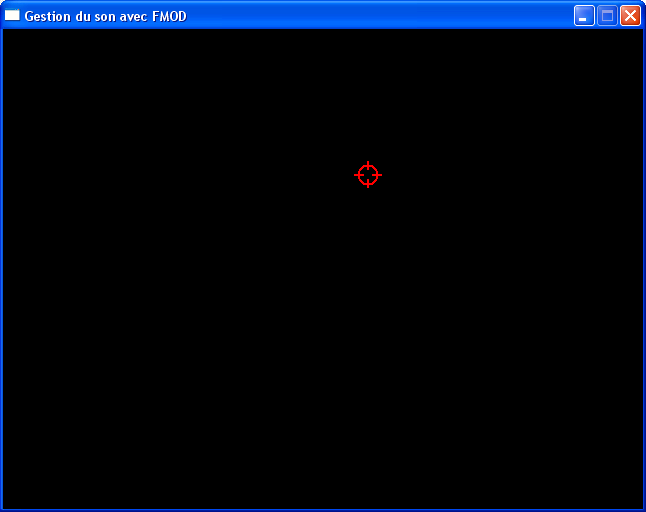
\includegraphics[width=0.8\textwidth]{Chapter_III-8_Window-aim}
\end{figure}

مشاهدة الفيديو هنا :\\
\url{https://openclassrooms.com/uploads/fr/ftp/mateo21/viseur.html}

 هنا، حمّلت
\textenglish{FMOD}
 قبل الـ\textenglish{SDL}
 و حررتها بعدها. لا توجد قواعد من ناحية الترتيب (كان بإمكاني القيام بالعكس). اخترتُ تحميل الـ\textenglish{SDL}
 و فتح النافذة بعد تحميل
\textenglish{FMOD}
 لكي تكون اللعبة جاهزة للاستعمال ما إن يتم فتح النافذة (و إلا كان بالإمكان أن تنتظر بعض الميلي ثواني ريثما يتم تحميل
\textenglish{FMOD}).\\
 و مع ذلك أنت حر باختيار الترتيب، هذه تفاصيل ليس إلا.

أعتقد أنني علّقت كفاية على الشفرة. لا يوجد فخ معيّن، و لا يوجد جديد يذكر. يمكننا أن نذكر الصعوبة "الصغيرة" التي تنص على لصق مركز المصوّب على مستوى مؤشّر الفأرة. يتم حساب وضعية الصورة بدلالة ذلك.

بالنسبة لمن لم يفهم الفرق بعد، سنرى ذلك الآن. بالمناسبة، لقد أعدت تفعيل الإظهار الخاص بالمؤشّر كي نرى كيف يتموضع المصوّب بالنسبة لمؤشّر الفأرة.

\begin{Table*}{3}
شفرة خاطئة (المصوب في وضعية خاطئة) &

\includegraphics[width=0.07\textwidth]{Chapter_III-8_Aim-misplaced} &
\parbox{0.45\textwidth}{\small\setLTR
\textenglish{\texttt{position.x = event.motion.x;\\
position.y = event.motion.y;}
}
\unsetLTR}
\\
شفرة صحيحة (المصوب في وضعية صحيحة) &

\includegraphics[width=0.07\textwidth]{Chapter_III-8_Aim-wellplaced} &
\parbox{0.45\textwidth}{\small\setLTR
\textenglish{\texttt{position.x = event.motion.x - (gunSight->w / 2);\\
position.y = event.motion.y - (gunSight->h / 2);}
}
\unsetLTR}
\\
\end{Table*}

\subsubsection{أفكار للتحسين}

هذه اللعبة تعتبر قاعدة للعبة إطلاق النار. لديك المصوّب، صوت إطلاق النار، لم يتبقّ لك سوى إظهار أو تمرير أعداء لكي يقوم اللاعب بإطلاق النار عليهم ثم يتم تسجيل النتيجة. كالعادة، عليك بالعمل وحدك. تريد صنع لعبة ؟ لا شيء يمنعك، بل لديك المستوى الكافي الآن، و لديك أيضاً شفرة مبدئية للعبة إطلاق النار ! ماذا تنتظر، صدقاً ؟ 

\begin{information}
طبعاً، منتديات
\href{http://www.siteduzero.com/forum-81-126-langage-c.html}{\textenglish{OpenClassrooms}}
ستساعدك في حال علقت في أيّ لحظة أثناء إنشائك للعبة. مواجهة الصعوبات أمر عادي مهما كان المستوى الذي أنت فيه.
\end{information}

\section{الموسيقى (\textenglish{WAV}، \textenglish{MP3}، \textenglish{OGG})}

نظرياً، يسمح العَلم
\InlineCode{FMOD\_CREATESAMPLE}
بتحميل أي صوت مهما كان، من ضمنها الصيغ المضغوطة
\textenglish{WAV}، \textenglish{MP3}، \textenglish{OGG}.
 المشكل يخصّ الأصوات "الطويلة"، أي الموسيقى.
 
في الواقع، تدوم الموسيقى كمعدّل من 3 إلى 4 دقائق. لكن، بهذا العلم، تحمّل الدالة\\
\InlineCode{FMOD\_System\_CreateSound}
كلّ الملف في الذاكرة (و النسخة غير المضغوطة هي التي ستتواجد في الذاكرة، فهذا يعني أنها ستأخذ حيّزاً كبيراً !).

إذا كان لديك صوت طويل المدّة (سنتكلّم عن "الموسيقى" من الآن و صاعداً)، سيكون من المستحسن أن نحمّلها بشكل تدفّقي
(\textenglish{streaming})،
يعني أن نحمّل منها أجزاء صغيرة في نفس الوقت الذي تشغّل فيه، هذا في الواقع ما تقوم به كلّ البرامج الخاصة بقراءة الأصوات.

\subsection{إيجاد الموسيقى}

ندخل هنا إلى أرضية ملغّمة، شائكة، بها متفجّرات (سمّها كما تريد).\\
في الواقع، أغلب الموسيقى و الأغاني التي نعرفها معنيّة بحقوق المؤلّف. حتى لو كتبت برنامجاً صغيراً، يجب أن تدفع رسوماً إلى الـ\textenglish{SACEM}
(في فرنسا على الأقل).

إذا، على غرار الموسيقى
\textenglish{MP3}
المحميّة بحقوق المؤلّف، ماذا يتبقّى لنا ؟\\
لحسن الحظ، توجد أغاني حرة من الحقوق ! يسمح أصحابها بنشر أغانيهم بشكل حرّ، إذا لا يوجد أي مشكل في استعمالها في برامجك.

\begin{warning}
إذا كان برنامجك تجاريا، يجب أن تتكلّم مع الفنان نفسه، فهناك من لا يقبل الاستعمالات التجارية لأغانيه. الأغنية حرّة الحقوق يمكن تنزيلها، نسخها و سماعها بشكل حرّ، لكن هذا لا يعني أنه بإمكاننا تحصيل المال على حساب الفنانين !
\end{warning}

حسناً السؤال هو : "أين نجد موسيقى حرّة ؟". يمكننا أن نجري بحثاً بالعبارة
"\textenglish{Free Music}"
في
\textenglish{Google}،
لكن هنا، هو ليس صديقنا هذه المرة. في الواقع، لنعرف لماذا، لقد كتبنا الكلمة
\textenglish{Free}
لكننا سنقع دائما على مواقع تطلب منا اشتراء الأغاني  !

لحسن الحظ، توجد مواقع تحتوي موسيقى حرة الحقوق. هنا أنصحك بالموقع الجيد
\textenglish{Jamendo}
لكنه ليس وحده الموجود في المجال.
\url{https://www.jamendo.com/}

يتم تقسيم الأغاني على حسب النمط. لديك الكثير من الخيارات، ستجد الجيد، السيء و الجيد جداً، و عديم الجودة. في الواقع، كلّ يعتمد على ذوقك و تقبّلك للأنماط المختلفة من الموسيقى. من المستحسن أن تختار موسيقى تشغّل في خلفية اللعبة و تكون متناسبة مع عالم اللعبة.

لمعلوماتك، توجد أغنية تنتمي إلى الألبوم
"\textenglish{Lies and Speeches}"
للمجموعة
"\textenglish{Hype}".
إذا أردت معرفة المزيد عنها، زر صفحتهم على الموقع
\textenglish{My Space} :
\url{http://www.myspace.com/hypemusic}

\begin{information}
متيقّن جداً أن الأذواق و الألوان لا مجال للنقاش فيهما. لا بأس باختيارك لأغنية أخرى إن كانت هذه لا تُعجبك.
\end{information}

لقد حمّلت إذاً الألبوم و سأستعمل أغنية
\textenglish{Home}
بصيغة
\textenglish{MP3}.\\
يمكنك تنزيلها مباشرة إذا أردت إختبار الشفرة في نفس الوقت معي. هذه من ميزات الموسيقى الحرة : يمكننا نسخها، توزيعها بشكل حر و لهذا لن نكون منزعجين.

\subsection{الخطوات الواجب اتّباعها لتشغيل الموسيقى}

الاختلاف الوحيد هو العَلم المُعطى للدالة
\InlineCode{FMOD\_System\_CreateSound}.\\
في عوض أن نعطيها العَلم
\InlineCode{FMOD\_CREATESAMPLE}،
نعطيها الأعلام :
\InlineCode{FMOD\_SOFTWARE}، \InlineCode{FMOD\_2D} و \InlineCode{FMOD\_CREATESTREAM}.\\
لا تنتظر كثيراً أن أشرح لك بشكل موسّع معاني هذه الأعلام، العَلم الذي يهمّنا أكثر هو
\InlineCode{FMOD\_CREATESTREAM}
لأنه يطلب من
\textenglish{FMOD}
تحميل الموسيقى جزءاً بجزء.

لكي نستعمل كلّ هذه الأعلام في نفس الوقت، نستعمل العامل المنطقي
\InlineCode{|}
بهذه الطريقة :

\begin{Csource}
FMOD_System_CreateSound(system, "my_music.mp3", FMOD_SOFTWARE | FMOD_2D | FMOD_CREATESTREAM, 0, &sound);
\end{Csource}

هكذا هو العمل  !\\
لكن هذا ليس كلّ شيء. في حالة موسيقى، سيكون من الجيد أن نعرف كيف نغيّر من قوّة الصوت، نتحكّم في إعادة الأغنية مرات عديدة، إيقافها مؤقّتا، أو حتى إيقافها كلياً. هذا النوع من الأشياء ما سنراه الآن. لكن قبل هذا، سنحتاج أن نعمل على القنوات بشكل مباشر.

\subsubsection{استرجاع قناة أو مجموعة من القنوات}

في نسخ سابقة من المكتبة
\textenglish{FMOD}،
رقم الهويّة البسيط لقناة يكفي لكي يغيّر قوّة الصوت أو إيقاف أغنية مؤقّتا.\\
طرأ تغيير صغير منذ
\textenglish{FMOD Ex} :
من خلال رقم القناة، نستعمل دالة توفّر لنا مؤشّراً نحو القناة. الفكرة تبقى نفسها، تتغيّر طريقة التنفيذ فقط.\\
يتم تعريف قناة كنوع
\InlineCode{FMOD\_CHANNEL}
و الدالة التي تسمح باسترجاع قناة إنطلاقاً من رقم الهوية هي
\InlineCode{FMOD\_System\_GetChannel}.\\
مثلاً، إذا كان لدي غرض نظامي و أردت استرجاع القناة رقم 9، يجب أن أكتب :

\begin{Csource}
FMOD_CHANNEL *channel;
FMOD_System_GetChannel(system, 9, &channel);
\end{Csource}

لا شيء أسهل من هذا !

\begin{itemize}
	\item المعامل الأول هو الغرض النظامي.
	\item المعامل الثاني هو رقم الهويّة الخاص بالقناة.
	\item المعامل الثالث هو عنوان المؤشّر الذي نريد تخزين المعلومة المُرادة فيه.
\end{itemize}

ما إن نتحصّل على مؤشّر القناة، يمكننا بسهولة التعامل مع الموسيقى (تغيير قوة الصوت، إيقاف الموسيقى مؤقّتا، \dots).

لاحظ أنه يمكننا أيضاً استرجاع مجموعة كاملة من القنوات في مؤشّر واحد : بهذا نتجنّب أن نقوم بنفس العملية من أجل كلّ قناة مختلفة.\\
نوع مجموعة القنوات هو
\InlineCode{FMOD\_CHANNELGROUP}
وواحدة من الدوال التي تهمّنا أكثر هي\\
\InlineCode{FMOD\_System\_GetMasterChannelGroup}
لأنها تسمح بالحصول على مؤشّر نحو كلّ القنوات المستعملة من طرف الغرض النظامي.\\
أسلوب عمل هذه الدالة مماثل لسابقتها.

\subsubsection{تغيير قوة الصوت}

لنغيّر قوة الصوت، يمكننا أن نقوم بذلك إما من أجل قناة محددة أو من أجل كلّ القنوات.\\
مثلاً، لكي نقوم بذلك من أجل كلّ القنوات، يجب أوّلاُ استرجاع المؤشّر نحو مجموعة القنوات، ثم استعمال الدالة
\InlineCode{FMOD\_ChannelGroup\_SetVolume}
ذات النموذج :

\begin{Csource}
FMOD_ChannelGroup_SetVolume 
FMOD_RESULT FMOD_ChannelGroup_SetVolume(
	FMOD_CHANNELGROUP *  channelgroup,  float  volume
);
\end{Csource}

المعامل
\InlineCode{channelgroup}
هو المعامل الذي نحن بصدد استرجاعه.\\
المعامل
\InlineCode{volume}
من نوع
\InlineCode{float}،
حيث $ 0.0 $ توافق المستوى الصامت و $ 1.0  $ توافق قراءة بكامل قوّة الصوت (هذه القيمة هي القيمة المُختارة تلقائيا).

\subsubsection{إعادة تشغيل الأغنية}

غالباً ما نحتاج إلى إعادة تشغيل الموسيقى الخلفية. هذا تماما ما تقترحه الدالة
\InlineCode{FMOD\_Sound\_SetLoopCount}
و التي تأخذ معاملين :

\begin{itemize}
	\item المؤشّر نحو الأغنية.
	\item عدد المرات التي يجب فيها أن تتم إعادة قراءة الموسيقى. إذا وضعت القيمة $ 1 $، تتم إذا قراءة الأغنية مرتين. إذا وضعت قيمة سالبة (مثل $ -1 $)، تتم إعادة قراءة الأغنية إلى ما لانهاية.
\end{itemize}

بهذه الشفرة المصدرية، يتم تكرار الأغنية إلى ما لانهاية : 

\begin{Csource}
FMOD_Sound_SetLoopCount(music, -1);
\end{Csource}

\begin{critical}
 لكي تشتغل عملية إعادة التشغيل، يجب أن نبعث 
\InlineCode{FMOD\_LOOP\_NORMAL}
 كمعامل ثالث للدالة
\InlineCode{FMOD\_System\_CreateSound}.
\end{critical}

\subsubsection{إيقاف الموسيقى مؤقتا}

توجد هنا دالتان لكي نتعلّمهما :

\begin{itemize}
	\item \InlineCode{FMOD\_Channel\_GetPaused} :
	تشير ما إذا كانت الأغنية التي يتم تشغيلها حالياً في القناة المختارة في حالة متوقفة مؤقتا أم لا. تعطي القيمة "صحيح" للمتغير 
	\InlineCode{state}
	إذا كانت الأغنية متوقفة مؤقتا، و القيمة "خطأ" ما إن كانت تشتغل حالياً.
	\item \InlineCode{FMOD\_Channel\_SetPaused} :
	توقف الأغنية مؤقتا أو تعيد تشغيلها في القناة المشار إليها. أعطها القيمة 1 (صحيح) لإيقافها مؤقتا. و 0 (خطأ) لإعادة تفعيل القراءة.
\end{itemize}

هذه الشفرة المصدرية الخاصة بنافذة
\textenglish{SDL}
تقوم بإيقاف الأغنية مؤقتا إذا ضغطنا على الزر
\InlineCode{P}
من لوحة المفاتيح، و تعيد تفعيلها إذا ضغطنا مجدداً على
\InlineCode{P}.

\begin{Csource}
case SDL_KEYDOWN:
if (event.key.keysym.sym == SDLK_p) // If we press P
{
	FMOD_BOOL state;
	FMOD_Channel_GetPaused(channel, &state);
	if (state == 1) // if the music is paused
		FMOD_Channel_SetPaused(channel, 0); // We play it
	else // Else, the music is being played
		FMOD_Channel_SetPaused(channel, 1); // We pause it
}
break;
\end{Csource}

 إذا أردنا إعادة تطبيق نفس الأمر من أجل كلّ القنوات معاً، نستعمل الدالتين\\
\InlineCode{FMOD\_ChannelGroup\_GetPaused}
 و
\InlineCode{FMOD\_ChannelGroup\_SetPaused}،
الاختلاف الوحيد الذي يجب القيام به هو إعطاءها كمعامل
\InlineCode{FMOD\_CHANNELGROUP}
بدلاً عن 
\InlineCode{FMOD\_CHANNEL}.

\subsubsection{إيقاف التشغيل}

يكفي استدعاء
\InlineCode{FMOD\_Channel\_Stop}
لأجل إيقاف موسيقى في قناة ما، أو\\
\InlineCode{FMOD\_ChannelGroup\_Stop}
من أجل مجموعة من القنوات، نبعث لها على الترتيب المؤشر نحو القناة أو المؤشّر نحو مجموعة القنوات.

\subsubsection{و بالطبع أشياء أخرى}

يمكننا القيام بالكثير من الأشياء الأخرى، لكن لن أقوم بتعدادها كلّها هنا. يجب عليك قراءة الملفات التوجيهية~! و التي أنصحك بإلقاء نظرة عليها في حال ما احتجت الاطلاع على دوال أخرى.

\subsubsection{تحرير الذاكرة}

لكي نقوم بتفريغ الأغنية من الذاكرة، نستدعي الدالة
\InlineCode{FMOD\_Sound\_Release}
و نعطيها المؤشّر :

\begin{Csource}
FMOD_Sound_Release(music);
\end{Csource}

\subsection{الشفرة المصدرية الكاملة لقراءة ملف \textenglish{MP3}}

الشفرة أسفله تقدّم لنا برنامجاً يقوم بتشغيل الموسيقى
"\textenglish{Home}"
التي حصلنا عليها من الموقع
\textenglish{Jamendo}.\\
يتم تشغيل الموسيقى منذ بداية تشغيل البرنامج. يمكننا إيقاف الموسيقى مؤقتا بالضغط على
\InlineCode{P}.

\begin{Csource}
#include <stdlib.h>
#include <stdio.h>
#include <SDL/SDL.h>
#include <SDL/SDL_image.h>
#include <fmodex/fmod.h>
int main(int argc, char *argv[])
{
	SDL_Surface *screen = NULL, *wallet = NULL;
	SDL_Event event;
	SDL_Rect position;
	int cont = 1;
	FMOD_SYSTEM *system;
	FMOD_SOUND *music;
	FMOD_RESULT result;
	FMOD_System_Create(&system);
	FMOD_System_Init(system, 1, FMOD_INIT_NORMAL, NULL);
	// We open the music
	result = FMOD_System_CreateSound(system, "hype_home.mp3", FMOD_SOFTWARE | FMOD_2D  | FMOD_CREATESTREAM, 0, &music);
	// We check if it has been opened successfully (IMPORTANT) 
	if (result != FMOD_OK)
	{
		fprintf(stderr, "Can't read the mp3 file\n");
		exit(EXIT_FAILURE);
	}
	// We activate the music repetition infinitely
	FMOD_Sound_SetLoopCount(music, -1);
	// We play the music
	FMOD_System_PlaySound(system, FMOD_CHANNEL_FREE, music, 0, NULL);
	SDL_Init(SDL_INIT_VIDEO);
	screen = SDL_SetVideoMode(640, 480, 32, SDL_HWSURFACE | SDL_DOUBLEBUF);
	SDL_WM_SetCaption("Managing sound with FMOD", NULL);
	wallet = IMG_Load("hype_liesandspeeches.jpg");
	position.x = 0;
	position.y = 0;
	while (cont)
	{
		SDL_WaitEvent(&event);
		switch(event.type)
		{
			case SDL_QUIT:
			cont = 0;
			break;
			case SDL_KEYDOWN:
			if (event.key.keysym.sym == SDLK_p) // If we press P
			{
				FMOD_CHANNELGROUP *channel;
				FMOD_BOOL state;
				FMOD_System_GetMasterChannelGroup(system, &channel);
				FMOD_ChannelGroup_GetPaused(channel, &state);
				if (state) // If the music is paused
					FMOD_ChannelGroup_SetPaused(channel, 0); // We play it
				else // Else, the music is being played
					FMOD_ChannelGroup_SetPaused(channel, 1); // We pause it
			}
			break;
		}
		SDL_FillRect(screen, NULL, SDL_MapRGB(screen->format, 0, 0, 0));
		SDL_BlitSurface(wallet, NULL, screen, &position);
		SDL_Flip(screen);
	}
	FMOD_Sound_Release(music);
	FMOD_System_Close(system);
	FMOD_System_Release(system);
	SDL_FreeSurface(wallet);
	SDL_Quit();
	return EXIT_SUCCESS;
}
\end{Csource}

لكي لا تكون خلفية البرنامج مجرّد صورة سوداء استعملت صورة الألبوم كخلفيّة.

يمكنك مشاهدة الفيديو الذي يمثّل تشغيل البرنامج من هنا.

\textenglish{\url{https://openclassrooms.com/uploads/fr/ftp/mateo21/musique_hype.html} (730 Ko)}

\section*{ملخّص}

\begin{itemize}
	\item لدى الـ\textenglish{SDL}
	مزايا محدودة بالنسبة للصوت و يُنصح أن تتم الاستعانة بمكتبة مخصصة لتشغيل الصوت مثل
	\textenglish{FMOD}.
	\item نميّز بين نوعين من الصوت بالـ\textenglish{FMOD} :
	أصوات قصيرة (ضجيج الخطوات مثلا) و أصوات طويلة (موسيقى مثلاً).
	\item كلّ من هذين النوعين يُقرأ بنفس الدالة لكن بواسطة أعلام مختلفة كخيارات.
	\item تسمح
	\textenglish{FMOD}
	بتشغيل كثير من الأصوات في آن واحد بالإستعانة بالكثير من القنوات.
\end{itemize}
